
\documentclass[12pt,a4paper]{ctexrep}
\usepackage{amsmath,amssymb}
\usepackage{fontspec}
\xeCJKsetup{AutoFallBack = true}
\setCJKfallbackfamilyfont\CJKrmdefault{Malgun Gothic}[Scale=MatchLowercase]
\setCJKfallbackfamilyfont\CJKsfdefault{Malgun Gothic}[Scale=MatchLowercase]
\setCJKfallbackfamilyfont\CJKttdefault{Malgun Gothic}[Scale=MatchLowercase]
\usepackage[top=1.5cm,bottom=1.5cm,left=1cm,right=1cm,headheight=15pt]{geometry}
\usepackage{pdflscape}


\usepackage{hyperref}
\usepackage{graphicx}
\usepackage{tikz}
\usetikzlibrary{shapes.multipart, decorations.pathreplacing, arrows.meta, positioning, matrix, calc}
\usepackage{float}
\usepackage{booktabs}
\usepackage{tabularx}
\usepackage{tabulary}
\usepackage{pgfplots}
\pgfplotsset{compat=1.18}
\usepackage{setspace}
\usepackage{fancyhdr}
\usepackage{algorithm}
\usepackage{algpseudocode}

\onehalfspacing
\pagestyle{fancy}
\fancyhf{}
% \fancyhead[C]{数据结构}
% \fancyfoot[C]{\small \thepage}

\hypersetup{
    colorlinks=true,
    linkcolor=black,
    citecolor=black,
    urlcolor=blue
}

\title{\textbf{\huge 数据结构}}
\author{}
\date{}

\begin{document}

\clearpage
\thispagestyle{empty}
\vspace*{\fill}

\begin{center}
{\huge 数据结构}\\[0.8em]
{\large Data Structures \& Algorithms}\\[2.5em]
{\large MS Roslyn}\\[0.6em]
{\large \today}
\end{center}

\vspace{2.5em}

\begin{center}
{\bfseries 摘要}
\end{center}

\vspace{1em}

\begin{center}
本教程系统介绍数据结构的核心概念与经典算法，涵盖位置记数系统、数据系统与物理存储、线性结构与抽象数据类型、树与二叉树、图论，以及算法定义与渐近分析、经典算法与核心运算，并通过不同算法的对比帮助读者理解时间与空间复杂度之间的权衡。教程将抽象数据类型与具体实现相结合，为程序设计提供坚实的数据组织基础。
\end{center}

\vspace*{\fill}
\clearpage

\tableofcontents
\newpage

\clearpage
\chapter{Positional Numeral System}

在数学中，\textbf{$n$ 进制}（进位计数制，Positional Numeral System）是指用一组固定的符号来表示任意实数的计数方法。其严谨的数学形式化定义由以下三个核心要素构成：

\section{任意进制定义}

\subsection{基数与合法数码集 (Alphabet of Digits)}

设基数 $n$ 为一个大于 1 的正整数（$n \in \mathbb{Z}^+, n > 1$）。
该进制的\textbf{有限数码集合 $S_n$} 严格定义为：
$$S_n = \{ x \mid x \in \mathbb{N}, 0 \leq x < n \} = \{0, 1, 2, \dots, n-1\}$$

\subsection{离散数码序列 (Numeral Sequence)}

任意实数在 $n$ 进制下的形式化表达，是一个双向无穷的\textbf{离散数码序列}：
$$\{P_i\}_{i=-\infty}^{\infty}$$
其中，每一位上的数码必须满足严格约束：$\forall i \in \mathbb{Z}, P_i \in S_n$。

\textit{注：为保证映射的唯一性，通常规定最高有效位向左不包含无穷个连续的 $0$，且小数末尾不包含无穷个连续的数码 $(n-1)$。}

\subsection{按权展开映射 (Polynomial Expansion)}

将"数码序列"映射到实数轴上的"绝对数值 $y$"（$y \in \mathbb{R}$），是通过\textbf{位权级数求和}实现的双向映射：
$$y = \sum_{i=-\infty}^{\infty} P_i \cdot n^i$$

将该无穷级数以小数点（$i=0$）为分界展开，其标准数学形式为：
$$y = \dots + P_2 \cdot n^2 + P_1 \cdot n^1 + P_0 \cdot n^0 + P_{-1} \cdot n^{-1} + P_{-2} \cdot n^{-2} + \dots$$

\begin{itemize}
    \item \textbf{整数部分 ($i \geq 0$)}：位权为 $n^i$，对应的基数为正指数幂。
    \item \textbf{小数部分 ($i < 0$)}：位权为 $n^i$，对应的基数为负指数幂。
\end{itemize}

\newpage

\section{\texorpdfstring{任意进制转换定义 ($n \to m$)}{任意进制转换定义 (n 转 m)}}

将一个数从 \textbf{$n$ 进制} 转换到 \textbf{$m$ 进制}，在数学上是通过\textbf{值守恒公理}与\textbf{数码分离算子}来进行形式化表达的。

\subsection{转换核心公理：值守恒 (Value Conservation)}

进制转换的本质是\textbf{变换数码的形式，但保持数轴上的绝对值 $y$ 不变}。
设源进制为 $n$（数码为 $P_i$），目标进制为 $m$（数码为 $Q_j$），则数学映射关系严格表达为：
$$y = \sum_{i=-\infty}^{\infty} P_i \cdot n^i = \sum_{j=-\infty}^{\infty} Q_j \cdot m^j$$
其中：$P_i \in S_n$，$Q_j \in S_m$。

\subsection{数学求解算子：数码分离 (Digit Extraction Operator)}

已知绝对值 $y$，想要显式直接求解目标 $m$ 进制中任意第 $j$ 位上的数码 $Q_j$，数学上使用\textbf{向下取整算子 $\lfloor \dots \rfloor$} 和 \textbf{取模算子 $\bmod$} 表达：

\begin{itemize}
    \item \textbf{整数部分（第 $j$ 位数码，其中 $j \geq 0$）：}
    $$Q_j = \left\lfloor \frac{y}{m^j} \right\rfloor \bmod m$$
    \textit{（注：将值右移 $j$ 位，截去低位干扰后取模）}
    
    \item \textbf{小数部分（第 $j$ 位数码，其中 $j < 0$）：}
    $$Q_j = \left\lfloor y_{\text{fraction}} \cdot m^{-j} \right\rfloor \bmod m$$
    \textit{（注：$y_{\text{fraction}} = y - \lfloor y \rfloor$ 为纯小数部分。通过左移 $-j$ 位将目标小数位提到整数个位，取整后取模剥离）}
\end{itemize}

\newpage

\section{\texorpdfstring{数学算子应用示例 ($10 \to 2$ 进制)}{数学算子应用示例 (10 转 2 进制)}}

\textbf{【示例】} 将十进制数 $y = 11.625$ 转换为二进制（目标基数 $m = 2$）。

\subsection{\texorpdfstring{整数部分求解 ($y = 11$, 求解 $j \geq 0$ 的数码)}{(1) 整数部分求解 (y = 11, 求解 j >= 0 的数码)}}

\begin{itemize}
    \item \textbf{$j = 0$（个位）:}  
    $$Q_0 = \left\lfloor \frac{11}{2^0} \right\rfloor \bmod 2 = 11 \bmod 2 = 1$$
    \item \textbf{$j = 1$（十位/$2^1$位）:}  
    $$Q_1 = \left\lfloor \frac{11}{2^1} \right\rfloor \bmod 2 = \lfloor 5.5 \rfloor \bmod 2 = 5 \bmod 2 = 1$$
    \item \textbf{$j = 2$（百位/$2^2$位）:}  
    $$Q_2 = \left\lfloor \frac{11}{2^2} \right\rfloor \bmod 2 = \lfloor 2.75 \rfloor \bmod 2 = 2 \bmod 2 = 0$$
    \item \textbf{$j = 3$（千位/$2^3$位）:}  
    $$Q_3 = \left\lfloor \frac{11}{2^3} \right\rfloor \bmod 2 = \lfloor 1.375 \rfloor \bmod 2 = 1 \bmod 2 = 1$$
    \item \textbf{$j = 4$:} $\left\lfloor \frac{11}{2^4} \right\rfloor = 0$，计算终止。  
    \textbf{得出整数部分：} $(11)_{10} = (Q_3 Q_2 Q_1 Q_0)_2 = (1011)_2$
\end{itemize}

\subsection{\texorpdfstring{小数部分求解 ($y_f = 0.625$, 求解 $j < 0$ 的数码)}{(2) 小数部分求解 (yf = 0.625, 求解 j < 0 的数码)}}

\begin{itemize}
    \item \textbf{$j = -1$（十分位/$2^{-1}$位）:}  
    $$Q_{-1} = \left\lfloor 0.625 \cdot 2^{-(-1)} \right\rfloor \bmod 2 = \lfloor 1.25 \rfloor \bmod 2 = 1 \bmod 2 = 1$$
    \item \textbf{$j = -2$（百分位/$2^{-2}$位）:}  
    $$Q_{-2} = \left\lfloor 0.625 \cdot 2^{-(-2)} \right\rfloor \bmod 2 = \lfloor 2.5 \rfloor \bmod 2 = 2 \bmod 2 = 0$$
    \item \textbf{$j = -3$（千分位/$2^{-3}$位）:}  
    $$Q_{-3} = \left\lfloor 0.625 \cdot 2^{-(-3)} \right\rfloor \bmod 2 = \lfloor 5.0 \rfloor \bmod 2 = 5 \bmod 2 = 1$$
    \item \textbf{$j = -4$:} 小数部分已被完全提取，后续结果均为 $0$，计算终止。

    \textbf{得出小数部分：} $(0.625)_{10} = (0.Q_{-1} Q_{-2} Q_{-3})_2 = (0.101)_2$
\end{itemize}

\subsection{最终值守恒合并}

$$\sum_{j=-3}^{3} Q_j \cdot 2^j = 1\cdot2^3 + 0\cdot2^2 + 1\cdot2^1 + 1\cdot2^0 + 1\cdot2^{-1} + 0\cdot2^{-2} + 1\cdot2^{-3} = 11.625$$
确定最终转换结果：$(11.625)_{10} = (1011.101)_2$

\section{算法级数轴递推（计算机实现逻辑的状态转移方程）}

在计算机实际运行中，如果直接对高维幂次 $m^j$ 进行直接计算（如前面的直接算子），会带来极高的\textbf{空间复杂度与浮点数精度误差}。为了让硬件高效执行，必须将静态的数学公式转化为\textbf{单步迭代的递推状态转移方程}。

这便是计算机中经典的 \textbf{"商与余数递推（除基取余法）"} 与 \textbf{"积与整数递推（乘基取整法）"}。

\subsection{整数项递推：商与余数 (Division-Remainder Iteration)}

此算法用于处理\textbf{整数部分}（$j \geq 0$）。它通过引入中间状态变量 $y_j$，在每一步循环中只做一次单步除法，从而把全局计算降维到局部计算。

\subsubsection{(1) 状态转移方程组}
$$\begin{cases}
Q_j = y_j \bmod m & \text{（状态输出：当前步的数码）} \\
y_{j+1} = \left\lfloor \frac{y_j}{m} \right\rfloor & \text{（状态转移：更新下一步的被除数）}
\end{cases}$$
\begin{itemize}
    \item \textbf{初始状态}：$y_0 = \lfloor y \rfloor$ （即原始数值的纯整数部分）。
    \item \textbf{终止条件}：当新状态 $y_{j+1} = 0$ 时，算法迭代停止。
\end{itemize}

\subsubsection{(2) 核心原理解析}
\begin{itemize}
    \item \textbf{$Q_j = y_j \bmod m$}：因为任意整数都可以写成 $y_j = k \cdot m + Q_j$ 的形式，所以对 $m$ 取模可以直接隔离出当前最低位（末尾）的数码。
    \item \textbf{$y_{j+1} = \left\lfloor \frac{y_j}{m} \right\rfloor$}：将当前数字整体向右移一位（抹去刚刚已经提取出的末尾数码），其商作为新的状态输入到下一轮循环中。
    \item \textbf{数码产出顺序}：由于我们是从个位开始向左剥离，因此数码的产出顺序是\textbf{从低位到高位}（即 $Q_0 \to Q_1 \to Q_2 \dots$）。计算机输出时需要逆序排列。
\end{itemize}

\subsection{小数项递推：积与整数 (Multiplication-Integer Iteration)}

此算法用于处理\textbf{小数部分}（$j < 0$）。由于小数点的右侧代表负指数幂（$\frac{1}{m}, \frac{1}{m^2}$），我们需要通过"放大"而非"缩小"来提取数码。

\subsubsection{(1) 状态转移方程组}
$$\begin{cases}
Q_j = \lfloor y_j \cdot m \rfloor & \text{（状态输出：当前步的数码）} \\
y_{j-1} = (y_j \cdot m) - Q_j & \text{（状态转移：更新下一步的纯小数）}
\end{cases}$$
\begin{itemize}
    \item \textbf{初始状态}：$y_{-1} = y - \lfloor y \rfloor$ （即原始数值的纯小数部分）。
    \item \textbf{终止条件}：新状态 $y_{j-1} = 0$（即小数部分完全被榨干清零）或达到指定的计算机最高精度步数。
\end{itemize}

\subsubsection{(2) 核心原理解析}
\begin{itemize}
    \item \textbf{$Q_j = \lfloor y_j \cdot m \rfloor$}：由于 $y_j$ 是一个处于 $[0, 1)$ 区间内的纯小数，将其乘以基数 $m$ 后，其原本在小数点后第一位的数字会被放大到整数部分（个位），通过向下取整即可直接摘取。
    \item \textbf{$y_{j-1} = (y_j \cdot m) - Q_j$}：乘基之后，减去刚刚脱离出来的整数部分 $Q_j$，剩下的依然是一个纯小数。这个余下的纯小数作为新的状态，继续投入下一次放大。
    \item \textbf{数码产出顺序}：因为我们是从十分位开始向右逐位放大剥离，所以数码的产出顺序是\textbf{从高位到低位}（即 $Q_{-1} \to Q_{-2} \to Q_{-3} \dots$）。计算机输出时按常规正序拼接即可。
\end{itemize}

\clearpage
\chapter{Data System and Physical Storage}

本章自底向上探讨数据的数学本质：从比特域出发，经数、字符的解释协议，到线性表的物理组织。数学层只谈集合与映射，位宽、字节、语言类型均为实例化。

\section{最根本元起点}

\begin{itemize}
    \item \textbf{基本域}：$\mathbb{B} = \{0, 1\}$。
    \item \textbf{比特序列空间}：$\mathbb{B}^* = \bigcup_{n=0}^{\infty} \mathbb{B}^n$。所有存储对象均为 $\mathbb{B}^*$ 中的元素。
    \item \textbf{解释协议}：映射 $\mathcal{I}: \mathbb{B}^n \to \mathcal{D}$ 将比特流解释为数学对象 $\mathcal{D}$（整数、字符、地址等）。同一比特串在不同 $\mathcal{I}$ 下可解释为不同对象。
\end{itemize}

\section{数字体系 (Number)}

\subsection{\texorpdfstring{自然数 ($\mathbb{N}$)}{自然数 (N)}}

\begin{itemize}
    \item \textbf{对象}：$\mathbb{N} = \{0, 1, 2, \dots\}$。
    \item \textbf{不变式（定长无符号）}：$n$ 位 $b = b_{n-1}\dots b_0 \in \mathbb{B}^n$，解码
$$\mathcal{I}_{\mathbb{N}}(b) = \sum_{i=0}^{n-1} b_i 2^i, \quad \mathcal{I}_{\mathbb{N}}: \mathbb{B}^n \to [0, 2^n-1]$$
为双射，值域 $[0,2^n-1]$。
    \item \textbf{定理}：加法在环 $\mathbb{Z}_{2^n}$ 中封闭，溢出即模 $2^n$ 回绕。
    \item \textbf{实例化}：网页 \texttt{unsigned-int} 按 $y \gets \sum b_i2^i$ 逐位累加演示；$n=8$ 时 $y \in [0,255]$ 为实例。
\end{itemize}

\subsection{\texorpdfstring{整数 ($\mathbb{Z}$)}{整数 (Z)}}

\begin{itemize}
    \item \textbf{对象}：$\mathbb{Z} = \{\dots, -2, -1, 0, 1, 2, \dots\}$。
    \item \textbf{不变式（补码）}：$b = b_{n-1}\dots b_0 \in \mathbb{B}^n$，
$$\mathcal{I}_{\mathbb{Z}}(b) = -b_{n-1}2^{n-1} + \sum_{i=0}^{n-2} b_i2^i$$
符号位负权消除 $+0/-0$ 二义性。
    \item \textbf{定理}：$\mathcal{I}_{\mathbb{Z}}: \mathbb{B}^n \to [-2^{n-1}, 2^{n-1}-1]$ 为双射；同一比特加法器对 $\mathcal{I}_{\mathbb{N}}$ 与 $\mathcal{I}_{\mathbb{Z}}$ 均正确（模 $2^n$ 同构）。
    \item \textbf{实例化}：网页 \texttt{twos-complement} 演示符号位 $-2^{n-1}$ 与低位累加；$n=8$ 时 $[-128,127]$ 为实例。
\end{itemize}

\subsection{\texorpdfstring{实数/有理数 ($\mathbb{R} \to \mathbb{Q}_{\text{discrete}}$)}{实数/有理数 (R 到 Q discrete)}}

\textbf{物理事实}：离散状态机无法精确表示连续无理数，实数离散化为 $\mathbb{Q}_{\text{discrete}} \subset \mathbb{Q}$。

\begin{enumerate}
    \item \textbf{定点数 (Fixed-Point)}：$x = m \cdot B^{-f}$，$m \in \mathbb{Z}$，$f$ 固定。值域与精度由 $f$ 权衡。
    \item \textbf{浮点数 (Floating-Point)}：
    \begin{itemize}
        \item \textbf{通用形式}：$x = (-1)^s \cdot m \cdot 2^e$，$s \in \mathbb{B}$，$m$ 为尾数，$e$ 为指数。
        \item \textbf{IEEE 754 结构}：$n$ 位划分为 $[s \mid E \mid F]$，$k$ 为指数位宽，$p$ 为尾数位宽，偏置 $\text{Bias}=2^{k-1}-1$，$E_{\text{raw}} \in [0,2^k-1]$。
        \begin{itemize}
            \item $E_{\text{raw}}=0, F=0$：$\pm 0$。
            \item $E_{\text{raw}}=0, F\neq0$：非规格化 $x=(-1)^s\cdot (F/2^p)\cdot 2^{1-\text{Bias}}$。
            \item $1\le E_{\text{raw}}\le 2^k-2$：规格化 $x=(-1)^s\cdot (1+F/2^p)\cdot 2^{E_{\text{raw}}-\text{Bias}}$（隐含前导 $1$）。
            \item $E_{\text{raw}}=2^k-1, F=0$：$\pm\infty$；$F\neq0$：$\text{NaN}$。
        \end{itemize}
        \item \textbf{实例参数}：binary32 $k=8,p=23,\text{Bias}=127$；binary64 $k=11,p=52,\text{Bias}=1023$。
        \item \textbf{等价判定}：引入容差 $\epsilon>0$，$a\equiv_\epsilon b \iff |a-b|<\epsilon$，避免直接判等。
    \end{itemize}
\end{enumerate}

\begin{itemize}
    \item \textbf{实例化}：网页 \texttt{ieee754} 支持 binary32/64 编解码与分类演示；上述公式为数学层，位串布局为实例。
\end{itemize}

\section{字符体系 (Character)}

\begin{itemize}
    \item \textbf{对象}：有限字母表 $\Sigma$，字符串幺半群 $(\Sigma^*,\circ,\varepsilon)$。
\end{itemize}

\subsection{ANSI / ASCII}

\begin{itemize}
    \item \textbf{对象}：映射 $\phi: \{0,\dots,127\} \to \Sigma_{\text{ASCII}}$ 为双射，$|\Sigma_{\text{ASCII}}|=128$。
    \item \textbf{不变式}：$7$ 位码 $\in [0,127]$。
    \item \textbf{实例化}：存储实例将 $7$ 位以 $0xxxxxxx$ 置于 $1$ 字节（$8$ 位），最高位恒 $0$；网页 \texttt{character-encoding} 模式 \texttt{ascii} 演示该实例。
\end{itemize}

\subsection{Unicode 架构}
\begin{enumerate}
    \item \textbf{抽象字符集 (UCS)}：全局空间 $\mathcal{U}$，$c\in\mathcal{U}$ 对应唯一码点 $u\in\mathbb{N}$，记 $\text{U}+XXXX$。
    \item \textbf{编码方案 (UTF)}：$\psi: \mathcal{U}\to\mathbb{B}^*$ 具前缀可解码性。
    \begin{itemize}
        \item \textbf{UTF-8}：变长 $1$--$4$ 字节，
        \begin{center}
        \small
        $U+0000$--$007F$: $0xxxxxxx$; $U+0080$--$07FF$: $110xxxxx\;10xxxxxx$; $U+0800$--$FFFF$: $1110xxxx\;10xxxxxx\;10xxxxxx$; $U+10000$--$10FFFF$: $11110xxx\;10xxxxxx\;10xxxxxx\;10xxxxxx$
        \end{center}
        向下兼容 ASCII（首字节 $0$ 判单字节）。
        \item \textbf{UTF-16/32}：$\psi$ 的另两种实例化，码点到码元的定/变长映射。
    \end{itemize}
\end{enumerate}

\begin{itemize}
    \item \textbf{实例化}：网页 \texttt{character-encoding} 模式 \texttt{utf8} 按码点区间分步生成字节；字符字形与字节存储均为实例。
\end{itemize}

\section{物理存储结构：线性表（Linear List）}

线性表是有限序列 $L = \langle d_1, d_2, \dots, d_n \rangle$，$d_i \in \mathcal{D}$。

\subsection{顺序存储结构（顺序表 / 数组）}

\begin{itemize}
    \item \textbf{对象}：基址 $\beta$，元大小 $\sigma$，连续区间 $[\beta, \beta+n\sigma)$。
    \item \textbf{不变式（随机访问）}：$\text{Addr}(i)=\beta+i\sigma$，$0\le i<n$，时间 $O(1)$。
    \item \textbf{多维压平（行优先）}：$M\times N$ 矩阵逻辑 $(i,j)$ 映为 $\text{Addr}(i,j)=\beta+(iN+j)\sigma$；列优先为对偶实例。
\end{itemize}

\begin{figure}[H]
\centering
\begin{tikzpicture}[
    cell/.style={draw, minimum width=1.4cm, minimum height=0.8cm, font=\ttfamily},
    addr/.style={font=\small},
    arrow/.style={->, >=latex}
]
    \node[cell] (c0) at (0,0) {$d_0$};
    \node[cell] (c1) at (2.6,0) {$d_1$};
    \node[cell] (c2) at (5.2,0) {$d_2$};
    \node[cell] (c3) at (7.8,0) {$d_3$};
    \node[cell] (c4) at (10.4,0) {$\dots$};
    \draw[arrow] (c0.south) -- ++(0,-0.5) node[addr, below] {$\beta$};
    \draw[arrow] (c1.south) -- ++(0,-0.5) node[addr, below] {$\beta+\sigma$};
    \draw[arrow] (c2.south) -- ++(0,-0.5) node[addr, below] {$\beta+2\sigma$};
    \node[addr, anchor=west] at ($(c4.east)+(0.3,0)$) {$\leftarrow$ 物理地址连续，支持 $O(1)$ 随机访问};
\end{tikzpicture}
\caption{一维顺序表物理内存布局}
\label{fig:array_1d}
\end{figure}

\begin{figure}[H]
\centering
\begin{tikzpicture}[
    cell/.style={draw, minimum size=0.75cm, font=\ttfamily},
    bigcell/.style={draw, minimum width=1.1cm, minimum height=0.75cm, font=\ttfamily},
    arrow/.style={->, >=latex, thick},
    brace/.style={decorate, decoration={brace, amplitude=5pt, mirror}}
]
    \matrix (mlog) [matrix of nodes, nodes={cell}, column sep=-\pgflinewidth, row sep=-\pgflinewidth] {
        (0,0) & (0,1) & (0,2) \\
        (1,0) & (1,1) & (1,2) \\
    };
    \node[left=0.3cm of mlog, font=\bfseries] {逻辑结构};

    \draw[arrow] (mlog.south) -- ++(0,-0.7) node[midway, right, font=\small] {行优先压平};

    \matrix (mphy) [matrix of nodes, nodes={bigcell}, column sep=-\pgflinewidth, below=1.1cm of mlog.south] {
        (0,0) & (0,1) & (0,2) & (1,0) & (1,1) & (1,2) \\
    };
    \node[right=0.3cm of mphy, font=\bfseries] {物理内存排列};

    \draw[brace] (mphy-1-1.south west) -- (mphy-1-3.south east) node[midway, below=5pt, font=\small] {第 0 行};
    \draw[brace] (mphy-1-4.south west) -- (mphy-1-6.south east) node[midway, below=5pt, font=\small] {第 1 行};

    \node[font=\small] (base) at ($(mphy-1-1.south)+(0,-1.3)$) {$\beta$};
    \draw[arrow] (base.north) -- ($(mphy-1-1.south)+(0,-0.05)$);
\end{tikzpicture}
\caption{二维数组行优先 (Row-Major) 压平排列}
\label{fig:array_2d}
\end{figure}

\begin{itemize}
    \item \textbf{稀疏压缩}：$A\in\mathbb{R}^{M\times N}$，三元组 $\mathcal{T}=\{(i,j,A_{ij})\mid A_{ij}\neq0\}$，空间 $O(|\mathcal{T}|)$，检索需索引结构。
    \item \textbf{实例化}：网页 \texttt{sequential-list}、\texttt{matrix} 演示连续寻址与越界；行/列优先、稀疏三元组均为本映射的实例。
\end{itemize}

\subsection{链式存储结构（链表 / Link List）}

\begin{itemize}
    \item \textbf{对象}：节点 $n_k=(d_k,p_k)$，$p_k\in\text{Memory}\cup\{\emptyset\}$。
    \item \textbf{不变式}：$p_k=\text{Addr}(n_{k+1})$，$p_{\text{last}}=\emptyset$；双向加前驱，循环令 $p_{\text{last}}=\text{Addr}(n_1)$。
    \item \textbf{定理}：随机访问 $O(n)$，头插删 $O(1)$。
    \item \textbf{实例化}：网页 \texttt{linked-list}、\texttt{doubly-linked-list}、\texttt{circular-linked-list} 分别演示三类不变式的指针重写。
\end{itemize}

\begin{figure}[H]
\centering
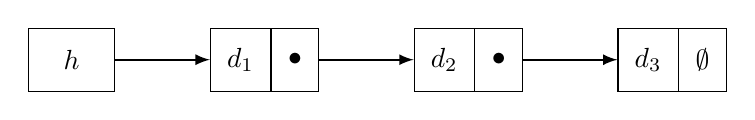
\begin{tikzpicture}[
    head/.style={draw, minimum width=1.1cm, minimum height=0.8cm, font=\ttfamily},
    lnode/.style={rectangle split, rectangle split horizontal, rectangle split parts=2,
                  rectangle split part align={center, center},
                  draw, minimum height=0.8cm, font=\ttfamily, inner sep=6pt},
    arrow/.style={->, >=latex, thick},
    node distance=1.2cm
]
    \node[head] (h) {$h$};
    \node[lnode, right=of h] (a) {$d_1$ \nodepart{two} $\bullet$};
    \node[lnode, right=of a] (b) {$d_2$ \nodepart{two} $\bullet$};
    \node[lnode, right=of b] (c) {$d_3$ \nodepart{two} $\emptyset$};

    \draw[arrow] (h.east) -- (a.west);
    \draw[arrow] (a.east) -- (b.west);
    \draw[arrow] (b.east) -- (c.west);
\end{tikzpicture}
\caption{单向链表 (Singly Linked List)}
\label{fig:linked_singly}
\end{figure}

\begin{figure}[H]
\centering
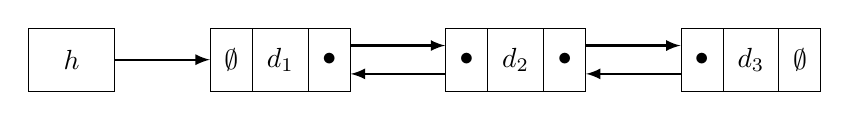
\begin{tikzpicture}[
    head/.style={draw, minimum width=1.1cm, minimum height=0.8cm, font=\ttfamily},
    dnode/.style={rectangle split, rectangle split horizontal, rectangle split parts=3,
                  rectangle split part align={center, center, center},
                  draw, minimum height=0.8cm, font=\ttfamily, inner sep=5pt},
    arrow/.style={->, >=latex, thick},
    node distance=1.2cm
]
    \node[head] (h) {$h$};
    \node[dnode, right=of h] (a) {$\emptyset$ \nodepart{two} $d_1$ \nodepart{three} $\bullet$};
    \node[dnode, right=of a] (b) {$\bullet$ \nodepart{two} $d_2$ \nodepart{three} $\bullet$};
    \node[dnode, right=of b] (c) {$\bullet$ \nodepart{two} $d_3$ \nodepart{three} $\emptyset$};

    \draw[arrow] (h.east) -- (a.west);
    \draw[arrow] ($(a.east)+(0,0.18)$) -- ($(b.west)+(0,0.18)$);
    \draw[arrow] ($(b.west)-(0,0.18)$) -- ($(a.east)-(0,0.18)$);
    \draw[arrow] ($(b.east)+(0,0.18)$) -- ($(c.west)+(0,0.18)$);
    \draw[arrow] ($(c.west)-(0,0.18)$) -- ($(b.east)-(0,0.18)$);
\end{tikzpicture}
\caption{双向链表 (Doubly Linked List)}
\label{fig:linked_doubly}
\end{figure}

\begin{figure}[H]
\centering
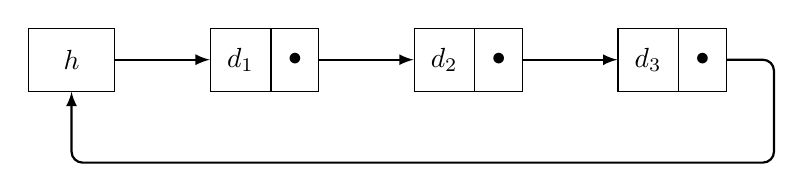
\begin{tikzpicture}[
    head/.style={draw, minimum width=1.1cm, minimum height=0.8cm, font=\ttfamily},
    lnode/.style={rectangle split, rectangle split horizontal, rectangle split parts=2,
                  rectangle split part align={center, center},
                  draw, minimum height=0.8cm, font=\ttfamily, inner sep=6pt},
    arrow/.style={->, >=latex, thick},
    node distance=1.2cm
]
    \node[head] (h) {$h$};
    \node[lnode, right=of h] (a) {$d_1$ \nodepart{two} $\bullet$};
    \node[lnode, right=of a] (b) {$d_2$ \nodepart{two} $\bullet$};
    \node[lnode, right=of b] (c) {$d_3$ \nodepart{two} $\bullet$};

    \draw[arrow] (h.east) -- (a.west);
    \draw[arrow] (a.east) -- (b.west);
    \draw[arrow] (b.east) -- (c.west);
    \coordinate (ret) at ($(h.south)+(0,-0.9)$);
    \draw[arrow, rounded corners=4pt] (c.east) -- ++(0.6,0) |- (ret) -- (h.south);
\end{tikzpicture}
\caption{循环链表 (Circular Linked List)}
\label{fig:linked_circular}
\end{figure}

\section{核心矛盾对比：顺序表 vs 链表}

\begin{table}[htbp]
\centering
\renewcommand{\arraystretch}{1.5}
\begin{tabulary}{\textwidth}{@{}CCC@{}}
\toprule
\textbf{特性维度} & \textbf{顺序存储（数组）} & \textbf{链式存储（链表）} \\
\midrule
\textbf{物理内存要求} & 连续区间 $[\beta,\beta+n\sigma)$ & 离散节点集合 $\{n_1,\dots,n_k\}$ \\
\textbf{元素访问} & $O(1)$：$\text{Addr}(i)=\beta+i\sigma$ & $O(n)$：指针链遍历 \\
\textbf{插入/删除} & $O(n)$：平移 $d_{i+1}\dots d_n$ & $O(1)$：重写常数个指针（已知前驱） \\
\textbf{空间代价} & 连续分配，扩容需 $O(n)$ 复制（摊还） & 额外指针 $O(n\sigma_p)$，但无扩容复制 \\
\bottomrule
\end{tabulary}
\end{table}

\begin{itemize}
    \item \textbf{实例化}：顺序表的连续分配与扩容、链表的指针开销均为分配策略的实例；数学代价不变。
\end{itemize}

\clearpage
\chapter{Linear Structures and Abstract Data Types}

本章按数学四段体组织：对象--公理/不变式--定理--实例化。代数规约与物理实现分层，\texttt{Error}/\texttt{Exception}、数组下标、指针结构体均为实例化。

\section{栈 (Stack)}

\subsection{代数定义}
栈 $S$ 是定义在元素集 $E$ 上的代数结构，由以下算子与公理刻画：
\begin{itemize}
    \item \textbf{构造算子}：
    \begin{itemize}
        \item $\text{empty}: \to S$ （空栈）
        \item $\text{push}: S \times E \to S$ （压入）
    \end{itemize}
    \item \textbf{观测算子}：
    \begin{itemize}
        \item $\text{pop}: S \to S \cup \{\bot\}$ （弹出，偏函数）
        \item $\text{top}: S \to E \cup \{\bot\}$ （栈顶，偏函数）
        \item $\text{isEmpty}: S \to \mathbb{B}$ （判空）
    \end{itemize}
\end{itemize}

\textbf{公理系统}（$\forall s \in S, e \in E$）：
\begin{enumerate}
    \item $\text{isEmpty}(\text{empty}) = \text{true}$
    \item $\text{isEmpty}(\text{push}(s, e)) = \text{false}$
    \item $\text{pop}(\text{push}(s, e)) = s$
    \item $\text{top}(\text{push}(s, e)) = e$
    \item $\text{pop}(\text{empty}) = \bot, \quad \text{top}(\text{empty}) = \bot$
\end{enumerate}

\begin{itemize}
    \item \textbf{实例化}：网页 \texttt{stack} 演示 \texttt{push}/\texttt{pop}/\texttt{top} 的帧序列；语言实例中 $\bot$ 实现为异常或错误码，数学层仅以偏函数表达。
\end{itemize}

\subsection{物理实现方案}
\begin{enumerate}
    \item \textbf{顺序栈（有界实例）}：$S_m$ 映射到 $A[0..m-1]$，$t\in\{-1,\dots,m-1\}$，不变式 $t<m-1$ 为 \texttt{push} 的定义域，$t\ge0$ 为 \texttt{pop} 的定义域。
    \item \textbf{链栈（无界实例）}：映射到单向链表，表头即栈顶，无容量上限，为 $S$ 的无界实例。
\end{enumerate}

\begin{algorithm}[H]
\caption{栈操作规约（有界顺序实例，数学层为偏函数）}
\begin{algorithmic}[1]
\State \textbf{状态}: $A[0..m-1]$, $t\gets-1$
\Procedure{Push}{$e$} \Comment{requires $t<m-1$}
    \State $t\gets t+1$; $A[t]\gets e$
\EndProcedure
\Procedure{Pop}{} \Comment{requires $t\ge0$}
    \State $e\gets A[t]$; $t\gets t-1$; \Return $e$
\EndProcedure
\end{algorithmic}
\end{algorithm}

\begin{itemize}
    \item \textbf{实例化注}：溢出/下溢 $t=m-1$/$t=-1$ 时数学上无定义（$\bot$）；语言实例以 \texttt{Error}、异常或返回值标记，网页 \texttt{stack} 即按此演示。
\end{itemize}

\begin{figure}[H]
\centering
\begin{tikzpicture}[
    cell/.style={draw, minimum width=1.4cm, minimum height=0.75cm, font=\ttfamily},
    arrow/.style={->, >=latex, thick},
    lbl/.style={font=\small}
]
    \node[cell] (a) at (0,0) {$d_1$};
    \node[cell] (b) at (0,0.75) {$d_2$};
    \node[cell] (c) at (0,1.5) {$d_3$};
    \node[cell, draw=none, minimum height=0.4cm] (d) at (0,2.25) {};
    \draw (d.south west) -- (d.north west);
    \draw (d.south east) -- (d.north east);
    \draw[arrow] (-2.2, 2.25) -- node[lbl, below] {$\text{push}(e)$} (d.west);
    \draw[arrow] (d.east) -- node[lbl, below] {$\text{pop}()$} (2.2, 2.25);
    \node[lbl, anchor=west] at ($(c.east)+(0.2,0)$) {$\leftarrow$ 栈顶 ($t$)};
    \node[lbl, anchor=west] at ($(a.east)+(0.2,0)$) {$\leftarrow$ 栈底};
\end{tikzpicture}
\caption{栈 (Stack) 逻辑模型}
\label{fig:stack_model}
\end{figure}

\section{队列 (Queue)}

\subsection{代数定义}
队列 $Q$ 是定义在 $E$ 上的代数结构：
\begin{itemize}
    \item \textbf{构造算子}：$\text{emptyQ}: \to Q$，$\text{enqueue}: Q \times E \to Q$
    \item \textbf{观测算子}：$\text{dequeue}: Q \to Q \cup \{\bot\}$，$\text{front}: Q \to E \cup \{\bot\}$，$\text{isEmptyQ}: Q \to \mathbb{B}$（均为偏函数，空队列上为 $\bot$）
\end{itemize}

\textbf{公理系统}（$\forall q \in Q, e \in E$）：
\begin{enumerate}
    \item $\text{isEmptyQ}(\text{emptyQ}) = \text{true}$
    \item $\text{dequeue}(\text{enqueue}(\text{emptyQ}, e)) = \text{emptyQ}$
    \item $\text{dequeue}(\text{enqueue}(\text{enqueue}(q, e_1), e_2)) = \text{enqueue}(\text{dequeue}(\text{enqueue}(q, e_1)), e_2)$
    \item $\text{front}(\text{enqueue}(\text{emptyQ}, e)) = e$
    \item 若 $\text{isEmptyQ}(q) = \text{false}$，则 $\text{front}(\text{enqueue}(q, e)) = \text{front}(q)$
\end{enumerate}

\subsection{循环队列 (Circular Queue)}
为消除假溢出，将数组索引映射到剩余类环 $\mathbb{Z}_m$。
\begin{itemize}
    \item \textbf{对象}：$Q[0..m-1]$, $f,r\in\mathbb{Z}_m$。
    \item \textbf{不变式}：$f\leftarrow(f+1)\bmod m$, $r\leftarrow(r+1)\bmod m$；队空 $r=f$，队满 $(r+1)\bmod m=f$（牺牲一槽位的不变式实例，其他实例以计数器区分）。
    \item \textbf{定理}：环上 \texttt{enqueue}/\texttt{dequeue} 均为 $O(1)$。
    \item \textbf{实例化}：网页 \texttt{queue} 演示普通与循环队列的指针帧；计数器方案为另一实例。
\end{itemize}

\begin{algorithm}[H]
\caption{循环队列规约（有界实例，数学层为偏函数）}
\begin{algorithmic}[1]
\State \textbf{状态}: $Q[0..m-1]$, $f\gets0, r\gets0$
\Procedure{Enqueue}{$e$} \Comment{requires $(r+1)\bmod m\neq f$}
    \State $Q[r]\gets e$; $r\gets(r+1)\bmod m$
\EndProcedure
\Procedure{Dequeue}{} \Comment{requires $r\neq f$}
    \State $e\gets Q[f]$; $f\gets(f+1)\bmod m$; \Return $e$
\EndProcedure
\end{algorithmic}
\end{algorithm}

\begin{itemize}
    \item \textbf{实例化注}：满/空判据的 \texttt{Error} 为语言实例的 $\bot$ 实现；数学层以定义域表达。
\end{itemize}

\begin{figure}[H]
\centering
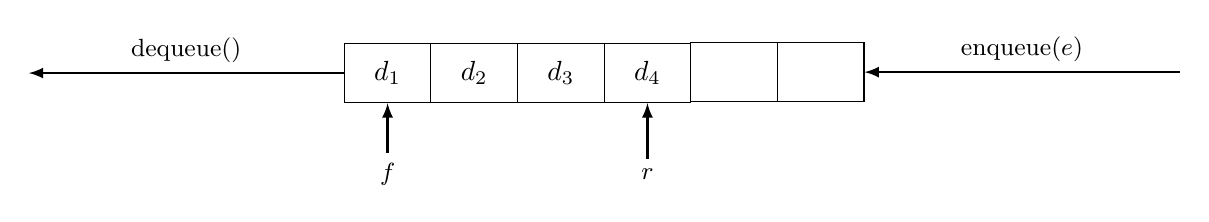
\begin{tikzpicture}[
    cell/.style={draw, minimum width=1.1cm, minimum height=0.75cm, font=\ttfamily},
    arrow/.style={->, >=latex, thick},
    lbl/.style={font=\small}
]
    \matrix (q) [matrix of nodes, nodes={cell}, column sep=-\pgflinewidth] {
        $d_1$ & $d_2$ & $d_3$ & $d_4$ & \phantom{A} & \phantom{A} \\
    };
    \draw[arrow] (q-1-1.west) -- ++(-4,0) node[lbl, midway, above] {$\text{dequeue}()$};
    \draw[arrow] ($(q-1-6.east)+(4,0)$) -- ++(-4,0) node[lbl, midway, above] {$\text{enqueue}(e)$};
    \node[lbl] (front) at ($(q-1-1.south)+(0,-0.9)$) {$f$};
    \draw[arrow] (front.north) -- (q-1-1.south);
    \node[lbl] (rear) at ($(q-1-4.south)+(0,-0.9)$) {$r$};
    \draw[arrow] (rear.north) -- (q-1-4.south);
\end{tikzpicture}
\caption{普通队列 (Queue)}
\label{fig:queue_model}
\end{figure}

\begin{figure}[H]
\centering
\begin{tikzpicture}[
    cell/.style={draw, minimum size=0.8cm, font=\ttfamily},
    arrow/.style={->, >=latex},
    lbl/.style={font=\small}
]
    \node[cell] (s5) at (90:1.8) {5};
    \node[cell] (s0) at (30:1.8) {0};
    \node[cell] (s1) at (-30:1.8) {1};
    \node[cell] (s2) at (-90:1.8) {2};
    \node[cell] (s3) at (-150:1.8) {3};
    \node[cell] (s4) at (150:1.8) {4};
    \draw[arrow] (s5) to[bend left=15] (s0);
    \draw[arrow] (s0) to[bend left=15] (s1);
    \draw[arrow] (s1) to[bend left=15] (s2);
    \draw[arrow] (s2) to[bend left=15] (s3);
    \draw[arrow] (s3) to[bend left=15] (s4);
    \draw[arrow] (s4) to[bend left=15] (s5);
    \node[lbl, anchor=west] at ($(s0.east)+(0.3,0)$) {$\leftarrow f$};
    \node[lbl, anchor=east] at ($(s3.west)+(-0.3,0)$) {$r \rightarrow$};
    \node[lbl, align=left, anchor=north west] at (3.2, -0.8) {
        队满判据 ($m=6$):\\
        $(r + 1) \bmod 6 = f$\\
        $(4 + 1) \bmod 6 = 5$
    };
\end{tikzpicture}
\caption{循环队列 (Circular Queue)}
\label{fig:queue_circular}
\end{figure}

\section{字符串 (String)}

\subsection{形式化定义}
\begin{itemize}
    \item \textbf{对象}：字母表 $\Sigma$ 有限非空。
    \item \textbf{字符串幺半群}：$\Sigma^* = \bigcup_{k=0}^{\infty} \Sigma^k$，空串 $\varepsilon\in\Sigma^0$，连接 $\circ: \Sigma^*\times\Sigma^*\to\Sigma^*$ 结合，$\varepsilon$ 为单位元。
    \item \textbf{不变式}：$|s\circ t| = |s|+|t|$，$|\varepsilon|=0$。
\end{itemize}

\begin{itemize}
    \item \textbf{物理实例}：底层以字符数组存储，边界以哨兵 $\#\notin\Sigma$ 界定。语言实例取 $\#=\backslash0$（C 字符串），数学层仅以 $\#\notin\Sigma$ 表达；网页 \texttt{string-ops} 演示连接、子串等幺半群操作。
\end{itemize}

\begin{figure}[H]
\centering
\begin{tikzpicture}[
    cell/.style={draw, minimum width=1.5cm, minimum height=0.75cm, font=\ttfamily},
    lbl/.style={font=\small}
]
    \matrix (str) [matrix of nodes, nodes={cell}, column sep=-\pgflinewidth] {
        $c_1$ & $c_2$ & $c_3$ & $\#$ \\
    };
    \node[lbl] at ($(str-1-1.south)+(0,-0.35)$) {0};
    \node[lbl] at ($(str-1-2.south)+(0,-0.35)$) {1};
    \node[lbl] at ($(str-1-3.south)+(0,-0.35)$) {2};
    \node[lbl] at ($(str-1-4.south)+(0,-0.35)$) {3};
    \node[lbl, anchor=west] at ($(str.east)+(0.3,0)$) {$\leftarrow s \in \Sigma^*$ 的物理映射（$\#\notin\Sigma$）};
\end{tikzpicture}
\caption{字符串物理存储布局}
\label{fig:string_layout}
\end{figure}

\section{高级映射与哈希表体系}

\subsection{字典 (Dictionary) / 映射 (Map)}
\begin{itemize}
    \item \textbf{对象}：偏函数 $\mathcal{M}: K \rightharpoonup V$，$\text{dom}(\mathcal{M})\subseteq K$。
    \item \textbf{不变式}：单射于键（$\mathcal{M}(k_1)=\mathcal{M}(k_2)\implies k_1=k_2$ 在值可逆时，或键唯一性由表保证）。
\end{itemize}

\subsection{哈希表 (Hash Table)}
通过 $h: K \to \mathbb{Z}_m$ 将键空间压缩至槽位 $\{0,\dots,m-1\}$。

\subsubsection{(1) 哈希函数}
\begin{itemize}
    \item \textbf{除留余数法}：$h(k)=k\bmod m$，$m$ 取质数以最小化冲突为实例化启发式。
    \item \textbf{理想哈希}：$\forall k_i\neq k_j\implies h(k_i)\neq h(k_j)$（鸽巢原理下仅当 $|K|\le m$ 可实现）。
\end{itemize}

\subsection{哈希碰撞 (Hash Collision)}
\subsubsection{(1) 碰撞必然性}
由鸽巢原理，若 $|K|>m$，则 $\exists k_i\neq k_j$ 使 $h(k_i)=h(k_j)$。

\begin{figure}[H]
\centering
\begin{tikzpicture}[
    keybox/.style={draw, minimum width=2.2cm, minimum height=0.7cm, font=\ttfamily},
    cell/.style={draw, minimum width=2cm, minimum height=0.7cm, font=\small},
    arrow/.style={->, >=latex, thick},
    lbl/.style={font=\small}
]
    \node[keybox] (k1) at (0, 0.55) {$k_1$};
    \node[keybox] (k2) at (0, -0.55) {$k_2$};
    \node[lbl, anchor=south] at ($(k1.north)+(0,0.15)$) {【输入键 $K$】};
    \node[cell] (s0) at (6.5, 0.7) {0: $\emptyset$};
    \node[cell, fill=yellow!25] (s1) at (6.5, 0) {1: $v$};
    \node[cell] (s2) at (6.5, -0.7) {2: $\emptyset$};
    \node[lbl, anchor=south] at ($(s0.north)+(0,0.3)$) {【槽位 $\mathbb{Z}_m$】};
    \draw[arrow] (k1.east) -- node[lbl, above, midway] {$h(k) \bmod m$} (s1.west);
    \draw[arrow] (k2.east) -- (s1.west);
    \node[lbl, red, anchor=west] at ($(s1.east)+(0.2,0)$) {$\leftarrow$ 碰撞：$h(k_1) = h(k_2)$};
\end{tikzpicture}
\caption{哈希碰撞三大核心要素模型}
\label{fig:hash_collision}
\end{figure}

\subsubsection{(2) 冲突解决方案}
\begin{enumerate}
    \item \textbf{开放寻址法 (Open Addressing)}
    \begin{itemize}
        \item 探测序列：$h_i(k) = (h(k) + \delta(i)) \bmod m$，所有槽位在主表中，冲突时按序列探测。
        \item \textbf{线性探测} $\delta(i)=i$：$h(k),h(k)+1,\dots$ 期望 $O(1+\alpha)$，但易主聚集。
        \item \textbf{二次探测} $\delta(i)=i^2$：$h(k),h(k)+1,h(k)+4,\dots$ 缓解主聚集；$m$ 为质数且 $\alpha<0.5$ 时可遍历。
        \item \textbf{双重散列} $h_i(k)=(h_1(k)+i\cdot h_2(k))\bmod m$，$h_2(k)\not\equiv0$，各键独立序列，最接近随机。
        \item \textbf{公共缺陷}：删除需墓碑标记，再散列为扩容实例。
        \item \textbf{实例化}：网页 \texttt{hash-table} 演示开放寻址的探测链；三者均为 $h_i$ 的实例化。
    \end{itemize}

    \item \textbf{链地址法 (Chaining)}
    \begin{itemize}
        \item 槽位 $i\in\mathbb{Z}_m$ 维护 $L_i=\{(k,v)\mid h(k)=i\}$。
        \item 期望 $O(1+\alpha)$，$\alpha=n/m$。
        \item \textbf{动态重构}：$|L_i|>\tau$ 时重构为平衡树（实例取红黑树），最坏 $O(\log n)$。
    \end{itemize}
\end{enumerate}

\begin{algorithm}[H]
\caption{哈希表查找与插入规约（以 $h_i$ 泛化，线性为实例）}
\begin{algorithmic}[1]
\State \textbf{状态}: $T[0..m-1]$, $h_i(k)$
\Procedure{Search}{$k$}
    \State $i\gets0$
    \Repeat
        \State $j\gets h_i(k)$ \Comment{实例：$(h(k)+i)\bmod m$ 为线性}
        \If{$T[j]=\emptyset$ \textbf{or} $T[j].key=k$} \Return $T[j]$ \EndIf
        \State $i\gets i+1$
    \Until{$i=m$}
    \State \Return $\bot$
\EndProcedure
\Procedure{Insert}{$k,v$}
    \State $item\gets\text{Search}(k)$
    \If{$item\neq\bot$} $item.value\gets v$
    \Else
        \State $i\gets0$; \While{True} $j\gets h_i(k)$; \If{$T[j]=\emptyset$} $T[j]\gets\langle k,v\rangle$; \Return \EndIf; $i\gets i+1$ \EndWhile
    \EndIf
\EndProcedure
\end{algorithmic}
\end{algorithm}

\begin{figure}[H]
\centering
\begin{tikzpicture}[
    cell/.style={draw, minimum width=1.1cm, minimum height=0.7cm, font=\ttfamily},
    kv/.style={draw, minimum width=1.9cm, minimum height=0.6cm, font=\small},
    arrow/.style={->, >=latex, thick},
    lbl/.style={font=\small}
]
    \matrix (bkt) [matrix of nodes, nodes={cell}, row sep=-\pgflinewidth] {
        0 \\
        1 \\
        2 \\
    };
    \node[lbl, anchor=south] at ($(bkt-1-1.north)+(0,0.15)$) {槽位 $i$};
    \node[kv, right=1.2cm of bkt-1-1] (ka) {$(k_1, v_1)$};
    \node[kv, right=0.5cm of ka] (kb) {$(k_2, v_2)$};
    \draw[arrow] (bkt-1-1.east) -- (ka.west);
    \draw[arrow] (ka.east) -- (kb.west);
    \node[lbl, anchor=west] at ($(kb.east)+(0.3,0)$) {$\to \emptyset$};
    \draw[arrow] (bkt-2-1.east) -- ++(1.2,0) node[lbl, anchor=west] {$\emptyset$};
    \node[draw, minimum width=2.2cm, minimum height=0.65cm, font=\small, right=1.2cm of bkt-3-1] (rbt) {红黑树};
    \draw[arrow] (bkt-3-1.east) -- (rbt.west);
    \node[lbl, anchor=north, align=center] at ($(rbt.south)+(0,-0.2)$) {
        （冲突数 $> \tau$ 时重构，\\
        检索复杂度 $O(\log n)$）
    };
\end{tikzpicture}
\caption{链地址法与动态重构模型}
\label{fig:hash_chaining}
\end{figure}

\begin{itemize}
    \item \textbf{实例化}：网页 \texttt{hash-table} 演示链地址与重构；三探测、墓碑、再散列均为本规约的实例化。
\end{itemize}

\clearpage
\chapter{Non-linear Structures I: Trees and Binary Trees}

树是一种一对多的非线性层次逻辑结构。在图论中，树被严密定义为：任意两个顶点间有且仅有一条路径的无环连通图。

\section{通用树的基础属性}

\begin{itemize}
    \item \textbf{形式化定义}：树 $T = (V, E)$，其中 $V$ 为有限顶点集，$E \subseteq V \times V$ 为边集，满足 $|E| = |V| - 1$ 且连通。
    \item \textbf{节点分类}：
    \begin{itemize}
        \item 根节点 (Root)：唯一入度为 0 的节点 $r \in V$。
        \item 叶子节点 (Leaf)：出度为 0 的节点集合 $L = \{ v \in V \mid \text{out-degree}(v) = 0 \}$。
        \item 分支节点 (Internal)：$I = V \setminus (L \cup \{r\})$。
    \end{itemize}
    \item \textbf{形态指标}：
    \begin{itemize}
        \item 度数 (Degree)：$\text{deg}(v) = |\{ u \mid (v, u) \in E \}|$。树的度 $D = \max_{v \in V} \text{deg}(v)$。
        \item 高度 (Height)：$H(T) = \max_{v \in V} \text{depth}(v)$。
    \end{itemize}
\end{itemize}

\section{二叉树 (Binary Tree) 及其形态特征}

\begin{itemize}
    \item \textbf{递归定义}：二叉树 $B$ 要么是空集 $\emptyset$，要么是一个三元组 $\langle d, L, R \rangle$，其中 $d$ 为根节点数据，$L$ 和 $R$ 为互不相交的二叉树（左子树与右子树）。
    \item \textbf{节点约束}：$\forall v \in V, \text{deg}(v) \in \{0, 1, 2\}$，且严格区分左右子树。
\end{itemize}

根据形态与平衡度，二叉树有以下经典状态：
\begin{enumerate}
    \item \textbf{偏斜树 (Skewed Tree)}：$\forall v, \text{deg}(v) \le 1$。退化为线性结构，检索复杂度 $O(n)$。
    \item \textbf{完全二叉树 (Complete Tree)}：节点按层序编号 $1 \dots n$，与满二叉树前 $n$ 个节点一一对应。
    \item \textbf{满二叉树 (Full Tree)}：$\forall v, \text{deg}(v) \in \{0, 2\}$，且所有叶子节点深度相同。
    \item \textbf{二叉搜索树 (BST)}：满足偏序关系 $\forall x \in L, x.val < d.val \land \forall y \in R, y.val > d.val$。
    \item \textbf{平衡二叉树 (AVL)}：$\forall v \in V, |H(L_v) - H(R_v)| \le 1$。
\end{enumerate}

\begin{figure}[H]
\centering
\begin{tikzpicture}[
    treenode/.style={circle, draw, minimum size=0.62cm, font=\ttfamily, inner sep=1pt},
    edge/.style={draw, thick},
    lbl/.style={font=\small\bfseries}
]
    \node[treenode] (sa) at (0,0) {A};
    \node[treenode] (sb) at (-0.55,-0.95) {B};
    \node[treenode] (sc) at (-1.1,-1.9) {C};
    \draw[edge] (sa) -- (sb);
    \draw[edge] (sb) -- (sc);
    \node[lbl] at (-0.55,-2.6) {偏斜退化树};

    \node[treenode] (ca) at (3.4,0) {A};
    \node[treenode] (cb) at (2.6,-0.95) {B};
    \node[treenode] (cc) at (4.2,-0.95) {C};
    \node[treenode] (cd) at (2.2,-1.9) {D};
    \node[treenode] (ce) at (3.0,-1.9) {E};
    \node[treenode] (cf) at (3.8,-1.9) {F};
    \draw[edge] (ca) -- (cb);
    \draw[edge] (ca) -- (cc);
    \draw[edge] (cb) -- (cd);
    \draw[edge] (cb) -- (ce);
    \draw[edge] (cc) -- (cf);
    \node[lbl] at (3.2,-2.6) {完全二叉树};

    \node[treenode] (fa) at (7.6,0) {A};
    \node[treenode] (fb) at (6.6,-0.95) {B};
    \node[treenode] (fc) at (8.6,-0.95) {C};
    \node[treenode] (fd) at (6.0,-1.9) {D};
    \node[treenode] (fe) at (7.2,-1.9) {E};
    \node[treenode] (ff) at (8.0,-1.9) {F};
    \node[treenode] (fg) at (9.2,-1.9) {G};
    \draw[edge] (fa) -- (fb);
    \draw[edge] (fa) -- (fc);
    \draw[edge] (fb) -- (fd);
    \draw[edge] (fb) -- (fe);
    \draw[edge] (fc) -- (ff);
    \draw[edge] (fc) -- (fg);
    \node[lbl] at (7.6,-2.6) {满二叉树};
\end{tikzpicture}
\caption{二叉树核心形态对比}
\label{fig:binary_tree_forms}
\end{figure}

\section{树的物理存储}

\begin{enumerate}
    \item \textbf{顺序存储法（完全二叉树）}
    \begin{itemize}
        \item 映射到数组 $A[0..n-1]$。
        \item 隐式纽带：$\forall i \in \{0, \dots, n-1\}$，
        \begin{itemize}
            \item 左子节点索引：$l(i) = 2i + 1$（若 $< n$）
            \item 右子节点索引：$r(i) = 2i + 2$（若 $< n$）
            \item 父节点索引：$p(i) = \lfloor (i-1)/2 \rfloor$（若 $i > 0$）
        \end{itemize}
    \end{itemize}
    \item \textbf{链式存储法（二叉链表）}
    \begin{itemize}
        \item 节点结构：$n = \langle lc, d, rc \rangle$，其中 $lc, rc \in \text{Node} \cup \{\emptyset\}$。
        \item 通用树转换（孩子兄弟表示法）：$n = \langle \text{firstChild}, d, \text{nextSibling} \rangle$。
    \end{itemize}
\end{enumerate}

\section{树的遍历 (Tree Traversal)}

将非线性结构 $T$ 映射为线性序列 $\sigma \in V^*$。

\subsection{递归遍历 (Recursive Traversal)}

\begin{algorithm}[H]
\caption{二叉树递归遍历伪代码 (Binary Tree Traversal)}
\begin{algorithmic}[1]
\Procedure{Preorder}{$u$} \Comment{前序遍历}
    \If{$u = \emptyset$} \State \Return \EndIf
    \State \textbf{Visit}($u$)
    \State \text{Preorder}($u.\text{left}$)
    \State \text{Preorder}($u.\text{right}$)
\EndProcedure
\Procedure{Inorder}{$u$} \Comment{中序遍历}
    \If{$u = \emptyset$} \State \Return \EndIf
    \State \text{Inorder}($u.\text{left}$)
    \State \textbf{Visit}($u$)
    \State \text{Inorder}($u.\text{right}$)
\EndProcedure
\Procedure{Postorder}{$u$} \Comment{后序遍历}
    \If{$u = \emptyset$} \State \Return \EndIf
    \State \text{Postorder}($u.\text{left}$)
    \State \text{Postorder}($u.\text{right}$)
    \State \textbf{Visit}($u$)
\EndProcedure
\end{algorithmic}
\end{algorithm}

\subsection{非递归遍历 (Iterative Traversal)}

利用显式栈 $S$ 模拟系统调用栈，消除递归开销。

\begin{algorithm}[H]
\caption{中序遍历迭代伪代码 (Iterative Inorder)}
\begin{algorithmic}[1]
\Procedure{InorderIterative}{$root$}
    \State $S \gets \emptyset$ \Comment{初始化空栈}
    \State $curr \gets root$
    \While{$curr \neq \emptyset$ \textbf{or} $S \neq \emptyset$}
        \While{$curr \neq \emptyset$}
            \State $\text{Push}(S, curr)$
            \State $curr \gets curr.\text{left}$
        \EndWhile
        \State $curr \gets \text{Pop}(S)$
        \State \textbf{Visit}($curr$)
        \State $curr \gets curr.\text{right}$
    \EndWhile
\EndProcedure
\end{algorithmic}
\end{algorithm}

\subsection{线索二叉树 (Threaded Binary Tree)}

为消除遍历时的栈空间开销 $O(H)$，利用空指针域存储遍历序中的前驱与后继。

\begin{itemize}
    \item \textbf{数学定义}：对于节点 $u$，定义标记位 $LTag, RTag \in \{0, 1\}$：
    \begin{itemize}
        \item 若 $u.\text{left} = \emptyset$，则 $u.\text{left} \gets \text{pre}(u)$（中序前驱），且 $LTag(u) = 1$。
        \item 若 $u.\text{right} = \emptyset$，则 $u.\text{right} \gets \text{succ}(u)$（中序后继），且 $RTag(u) = 1$。
    \end{itemize}
    \item \textbf{性质}：线索化后，遍历操作退化为线性扫描，空间复杂度降至 $O(1)$。
\end{itemize}

\subsection{遍历序列与树的唯一性}

\begin{enumerate}
    \item \textbf{唯一确定性定理}：
    \begin{itemize}
        \item \textbf{前序 + 中序} $\implies$ 唯一确定二叉树。
        \item \textbf{后序 + 中序} $\implies$ 唯一确定二叉树。
        \item \textbf{前序 + 后序} $\implies$ 仅当树为满二叉树时唯一确定，否则存在歧义（无法区分左右子树边界）。
    \end{itemize}
    \item \textbf{构造算法}：
\end{enumerate}

\begin{algorithm}[H]
\caption{由前序与中序序列构造二叉树}
\begin{algorithmic}[1]
\State \textbf{输入}: 前序序列 $P$, 中序序列 $I$
\Procedure{BuildTree}{$P, I$}
    \If{$P = \emptyset$ \textbf{or} $I = \emptyset$}
        \State \Return $\emptyset$
    \EndIf
    \State $root \gets P[0]$ \Comment{前序首元素为根}
    \State $k \gets \text{Index}(I, root)$ \Comment{在中序中定位根}
    \State $I_L \gets I[0..k-1]$, $I_R \gets I[k+1..|I|-1]$
    \State $P_L \gets P[1..|I_L|]$, $P_R \gets P[|I_L|+1..|P|-1]$
    \State $root.\text{left} \gets \text{BuildTree}(P_L, I_L)$
    \State $root.\text{right} \gets \text{BuildTree}(P_R, I_R)$
    \State \Return $root$
\EndProcedure
\end{algorithmic}
\end{algorithm}

\section{堆体系 (Heap)}

\begin{itemize}
    \item \textbf{定义}：完全二叉树 $T$ 满足堆序性质。
    \item \textbf{大顶堆 (Max Heap)}：$\forall v \in V, v.val \ge \text{leftChild}(v).val \land v.val \ge \text{rightChild}(v).val$。
    \item \textbf{小顶堆 (Min Heap)}：$\forall v \in V, v.val \le \text{leftChild}(v).val \land v.val \le \text{rightChild}(v).val$。
    \item \textbf{功能}：提供 $O(1)$ 的最值访问与 $O(\log n)$ 的动态插入/删除，是优先队列的物理实现。
\end{itemize}

\begin{algorithm}[H]
\caption{堆下滤操作伪代码 (Sift-Down for Max Heap)}
\begin{algorithmic}[1]
\State \textbf{输入}: 数组 $A$, 节点索引 $i$, 堆大小 $n$
\Procedure{SiftDown}{$i, n$}
    \State $largest \gets i$
    \State $l \gets 2i + 1$ \Comment{左孩子}
    \State $r \gets 2i + 2$ \Comment{右孩子}
    \If{$l < n$ \textbf{and} $A[l] > A[largest]$}
        \State $largest \gets l$
    \EndIf
    \If{$r < n$ \textbf{and} $A[r] > A[largest]$}
        \State $largest \gets r$
    \EndIf
    \If{$largest \neq i$}
        \State \textbf{Swap}($A[i], A[largest]$)
        \State \text{SiftDown}($largest, n$) \Comment{递归下滤}
    \EndIf
\EndProcedure
\end{algorithmic}
\end{algorithm}

\clearpage
\chapter{Non-linear Structures II: Graph Theory}

图是一种多对多的网状逻辑结构，用于建模现实世界中复杂的关联网络。

\section{图的形式化定义}

图 $G$ 定义为二元组 $G = (V, E)$：
\begin{itemize}
    \item $V = \{v_1, v_2, \dots, v_n\}$ 为有限顶点集合。
    \item $E \subseteq V \times V$ 为边集合。
    \item 若 $E$ 为无序对集合 $\{\{u, v\} \mid u, v \in V\}$，则为无向图; 若为有序对集合 $\{(u, v) \mid u, v \in V\}$，则为有向图。
\end{itemize}

\textbf{扩展属性}：
\begin{itemize}
    \item \textbf{权重函数}：$w: E \to \mathbb{R}$，赋予每条边实数值。
    \item \textbf{邻接映射}：$N: V \to \mathcal{P}(V)$，其中 $N(u) = \{ v \mid (u, v) \in E \}$。
\end{itemize}

\section{边的拓扑分类}

\begin{enumerate}
    \item \textbf{有向无环图 (DAG)}：有向图且不存在序列 $\langle v_1, v_2, \dots, v_k \rangle$ 使得 $(v_i, v_{i+1}) \in E$ 且 $v_1 = v_k$。
    \item \textbf{连通图 (Connected Graph)}：无向图中 $\forall u, v \in V$，存在路径 $P = \langle u=x_0, x_1, \dots, x_k=v \rangle$ 使得 $(x_i, x_{i+1}) \in E$。
\end{enumerate}

\section{连通性深度分析}

\begin{itemize}
    \item \textbf{强连通 (Strongly Connected)}：有向图中 $\forall u, v \in V$，存在 $u \to v$ 路径且存在 $v \to u$ 路径。
    \item \textbf{弱连通 (Weakly Connected)}：忽略边方向后形成的无向图是连通的。
    \item \textbf{桥 (Bridge)}：边 $e \in E$ 为桥 $\iff$ 移除 $e$ 后图的连通分量数增加，即 $G' = (V, E \setminus \{e\})$ 不连通。
\end{itemize}

\begin{figure}[H]
\centering
\begin{tikzpicture}[
    gnode/.style={circle, draw, minimum size=0.62cm, font=\ttfamily, inner sep=1pt},
    dedge/.style={->, >=latex, thick},
    uedge/.style={draw, thick},
    lbl/.style={font=\small\bfseries}
]
    \node[gnode] (a) at (0,0) {A};
    \node[gnode] (b) at (2.2,0) {B};
    \node[gnode] (c) at (0,-2.2) {C};
    \node[gnode] (d) at (2.2,-2.2) {D};
    \draw[dedge] ($(a.east)+(0,0.12)$) -- ($(b.west)+(0,0.12)$);
    \draw[dedge] ($(b.west)-(0,0.12)$) -- ($(a.east)-(0,0.12)$);
    \draw[dedge] (a) -- (c);
    \draw[dedge] (c) -- (d);
    \draw[dedge] (d) -- (b);
    \node[lbl] at (1.1,-3.0) {强连通有向图};

    \node[gnode] (a2) at (5.5,0) {A};
    \node[gnode] (b2) at (7.5,0) {B};
    \node[gnode] (c2) at (6.5,-1.7) {C};
    \draw[uedge] (a2) -- (b2);
    \draw[uedge] (a2) -- (c2);
    \draw[uedge] (b2) -- (c2);
    \node[gnode] (x2) at (10.5,0) {X};
    \node[gnode] (y2) at (12.5,0) {Y};
    \node[gnode] (z2) at (11.5,-1.7) {Z};
    \draw[uedge] (x2) -- (y2);
    \draw[uedge] (x2) -- (z2);
    \draw[uedge] (y2) -- (z2);
    \draw[uedge, double, thick] (c2) -- (z2)
        node[midway, below=2pt, font=\small] {桥 $e$：$G-e$ 不连通};
    \node[lbl] at (9,-3.0) {包含``桥''的断连风险图};
\end{tikzpicture}
\caption{图的位置连通性形态与``桥''}
\label{fig:graph_connectivity}
\end{figure}

\section{图的降维与拓扑排序}

\begin{algorithm}[H]
\caption{图遍历伪代码 (Graph Traversal)}
\begin{algorithmic}[1]
\State \textbf{全局变量}: $\text{Visited} \subseteq V$ (初始为 $\emptyset$)
\Procedure{BFS}{$s$} \Comment{广度优先搜索}
    \State $Q \gets \{s\}$
    \State $\text{Visited} \gets \text{Visited} \cup \{s\}$
    \While{$Q \neq \emptyset$}
        \State $u \gets \text{Dequeue}(Q)$
        \State \textbf{Visit}($u$)
        \ForAll{$v \in N(u) \setminus \text{Visited}$}
            \State $\text{Visited} \gets \text{Visited} \cup \{v\}$
            \State $\text{Enqueue}(Q, v)$
        \EndFor
    \EndWhile
\EndProcedure
\Procedure{DFS}{$u$} \Comment{深度优先搜索}
    \State $\text{Visited} \gets \text{Visited} \cup \{u\}$
    \State \textbf{Visit}($u$)
    \ForAll{$v \in N(u) \setminus \text{Visited}$}
        \State \text{DFS}($v$)
    \EndFor
\EndProcedure
\end{algorithmic}
\end{algorithm}

\begin{itemize}
    \item \textbf{拓扑排序 (Topological Sort)}：
    \begin{itemize}
        \item 对象：DAG。
        \item 目标：构造线性序列 $\sigma = \langle v_1, \dots, v_n \rangle$ 使得 $\forall (u, v) \in E$，若 $u=v_i, v=v_j$，则 $i < j$。
    \end{itemize}
\end{itemize}

\section{图的物理存储实现}

\begin{enumerate}
    \item \textbf{邻接矩阵 (Adjacency Matrix)}
    \begin{itemize}
        \item 定义：$A \in \{0, 1\}^{n \times n}$，其中 $A_{ij} = 1 \iff (v_i, v_j) \in E$。
        \item 带权图：$A_{ij} = w(v_i, v_j)$ 或 $\infty$。
        \item 空间复杂度：$O(|V|^2)$，适合稠密图。
    \end{itemize}
    \item \textbf{邻接表 (Adjacency List)}
    \begin{itemize}
        \item 定义：数组 $\text{Adj}[1..n]$，其中 $\text{Adj}[i] = \{ v \mid (v_i, v) \in E \}$ 以链表形式存储。
        \item 空间复杂度：$O(|V| + |E|)$，适合稀疏图。
    \end{itemize}
\end{enumerate}

\clearpage
\chapter{Algorithm Definition and Asymptotic Analysis}

本章探讨评价算法优劣的统一数学度量衡，建立时间与空间复杂度的渐进趋势评估模型。

\section{算法的定义与四大核心特征}

算法（Algorithm）是指解决特定问题的一组明确的、有穷的、可执行的指令序列。一个合格的算法必须具备以下四大核心特征：

\begin{enumerate}
    \item \textbf{有穷性（Finiteness）}：算法必须在执行有限个操作步骤后自动结束，不能陷入死循环，且每一步都应在有穷时间内完成。
    \item \textbf{确定性（Definiteness）}：算法中的指令每一步都必须有确切的含义，在任何条件下都具有唯一一条执行路径，不产生任何歧义。
    \item \textbf{可行性（Effectiveness）}：算法中涉及的所有操作均是最基础、可执行的，能够通过已经实现的底层基本运算在有限时间内准确运行。
    \item \textbf{输入/输出（Input / Output）}：一个算法拥有零个或多个输入（作为算法处理的初始物理量），并必然产生一个或多个输出（作为算法执行的结果回馈）。
\end{enumerate}

\section{算法的描述媒介}

根据“信息流动方向”与“面向对象（人或机器）”的不同，算法的描述主要分为两大阵营、四种流派：

\begin{itemize}
    \item \textbf{面向人类思维（人写人看）}：
    \begin{enumerate}
        \item \textbf{自然语言}：用人类日常语言描述。优点是通俗易懂，缺点是过于冗长且容易产生语义歧义。
        \item \textbf{流程图（Flowchart）}：利用图形化、具有严密逻辑关系的有向图来表达控制流。
        \item \textbf{伪代码（Pseudo-code）}：介于自然语言与编程语言之间。直接利用公式与控制流算子进行映射，具备接近代码的严密性，是学术界描述算法的标准媒介。
    \end{enumerate}
    \item \textbf{面向底层执行（人写机看）}：
    \begin{enumerate}
        \setcounter{enumi}{3}
        \item \textbf{高级编程语言}：如 C++、Java、Python 等。直接翻译为计算机硬件可以理解并编译运行的二进制指令。
    \end{enumerate}
\end{itemize}

\section{算法的时间复杂度 (Time Complexity)}

评价一个算法的优劣不能依靠绝对的计时。科学的评估方法是分析\textbf{输入规模 $n$ 与资源消耗规模之间的渐进趋势关系}。

\subsection{大 O 表示法的渐进上界定义}

大 O 符号用于寻求算法执行时间随着规模 $n$ 放大时的渐进上界。其严格数学定义为：若存在正连续常数 $c$ 和 $n_0$，使得当 $n \ge n_0$ 时，算法的实际运行时间 $T(n)$ 均满足：
$$T(n) \le c \cdot f(n)$$
则记作 $T(n) = O(f(n))$。它忽略了低阶项与常数系数，专注于长远增长趋势。

\subsection{复杂度阶数}

随着输入规模 $n$ 的爆炸式增长，不同复杂度阶数的资源消耗会产生明显的趋势分流。

\begin{figure}[H]
\centering
\begin{tikzpicture}
\begin{axis}[
    width=15cm, height=10cm,
    axis lines=left,
    axis line style={-latex, thick},
    xlabel={输入规模},
    ylabel={资源消耗},
    xmin=-2, xmax=45, ymin=-2.5, ymax=45,
    xtick={0,10,20,30,40},
    ytick={0,10,20,30,40},
    domain=0:40,
    samples=120,
    clip=false,
    every axis x label/.style={at={(ticklabel* cs:1)}, anchor=north},
    every axis y label/.style={at={(ticklabel* cs:1)}, anchor=south},
    legend style={draw=none},
]
    % 负半轴虚线延伸
    \draw[dashed, gray, thick] (axis cs:0,0) -- (axis cs:-2,0);
    \draw[dashed, gray, thick] (axis cs:0,0) -- (axis cs:0,-2.5);
    
    % O(1)
    \addplot[thick, gray] {1};
    \addplot[dashed, gray, domain=-2:0] {1};
    \node[anchor=west, font=\small, gray] at (axis cs:40,0.6) {$O(1)$ };
    % O(log n)
    \addplot[thick, green!60!black, domain=1:40] {log2(x)};
    \node[anchor=west, font=\small, green!60!black] at (axis cs:40,4.5) {$O(\log n)$ };
    % O(n)
    \addplot[thick, blue] {x};
    \addplot[dashed, blue, domain=-2:0] {x};
    \node[anchor=west, font=\small, blue] at (axis cs:40,38.5) {$O(n)$ };
    % O(n log n)
    \addplot[thick, cyan!60!black, domain=1:10] {x*log2(x)};
    \node[anchor=west, font=\small, cyan!60!black] at (axis cs:10,33.2) {$O(n \log n)$ };
    % O(n^2)
    \addplot[thick, magenta!80!black, domain=0:6.32] {x^2};
    \addplot[dashed, magenta!80!black, domain=-2:0] {x^2};
    \node[anchor=south west, font=\small, magenta!80!black] at (axis cs:6,38) {$O(n^2)$ };
    % O(2^n)
    \addplot[thick, red, domain=0:5.32] {2^x};
    \addplot[dashed, red, domain=-2:0] {2^x};
    \node[anchor=south west, font=\small, red] at (axis cs:1,35) {$O(2^n)$ };
    % O(n!) - 严格经过整数点并用平滑曲线连接
    \addplot[thick, red!60!black, samples at={0,1,2,3,4}, smooth] {factorial(x)};
    \node[anchor=south west, font=\small, red!60!black] at (axis cs:0,20) {$O(n!)$ };
\end{axis}
\end{tikzpicture}
\caption{大 O 渐进曲线趋势对比}
\label{fig:big_o_curves}
\end{figure}

\subsection{复杂度组合乘法原理}

当算法的各个模块相互嵌套或串联时，其大 O 符号满足乘法运算法则：
$$O(a) \cdot O(b) = O(a \cdot b)$$

\section{算法的空间复杂度 (Space Complexity)}

空间复杂度用于衡量随着输入规模 $n$ 的扩大，算法运行期间\textbf{额外占用的辅助存储空间}的增幅趋势。

\subsection{\texorpdfstring{$O(1)$}{O(1)} 常数级辅助空间（In-place 原地置换）}

算法在原输入数据的存储空间上直接进行修改与操作。整个过程不需要开辟随 $n$ 增长的新空间，仅需要常数个辅助变量用于临时中转。

\begin{figure}[H]
\centering
\begin{tikzpicture}[
    cell/.style={draw, minimum width=1.4cm, minimum height=0.75cm, font=\ttfamily},
    lbl/.style={font=\small}
]
    \matrix (arr) [matrix of nodes, nodes={cell}, column sep=-\pgflinewidth] {
        $d_1$ & $d_2$ & $d_3$ & $d_4$ \\
    };
    \node[lbl, anchor=south west] at ($(arr.north west)+(0,0.15)$) {原数组 $A$:};
    \draw[<->, >=latex, thick]
        ($(arr-1-1.south)+(0,-0.25)$) to[bend right=35]
        node[midway, below, lbl] {交换}
        ($(arr-1-2.south)+(0,-0.25)$);
    \node[lbl, anchor=north west, align=left] at ($(arr.south west)+(0,-1.0)$) {
        $\longrightarrow$ 借助常数槽位 $\tau$ 临时中转\\
        （辅助空间 $O(1)$）
    };
\end{tikzpicture}
\caption{原地置换 (Swap In-place) 内存状态机模型}
\label{fig:space_o1}
\end{figure}

\subsection{\texorpdfstring{$O(n)$}{O(n)} 线性级辅助空间（Clone 副本生成）}

在算法执行期间（如为了保持原数据不被破坏，或者为了进行高效率的哈希映射），必须在物理内存中动态生成一份与原输入规模等大的副本（Clone）。其开辟的内存槽位随 $n$ 同步线性增长。

\begin{figure}[H]
\centering
\begin{tikzpicture}[
    cell/.style={draw, minimum width=1.4cm, minimum height=0.75cm, font=\ttfamily},
    lbl/.style={font=\small}
]
    \matrix (src) [matrix of nodes, nodes={cell}, column sep=-\pgflinewidth] {
        $d_1$ & $d_2$ & $d_3$ & $d_4$ \\
    };
    \node[lbl, anchor=south west] at ($(src.north west)+(0,0.15)$) {原数组 $A$（规模 $n$）:};
    \matrix (dst) [matrix of nodes, nodes={cell}, column sep=-\pgflinewidth, below=1.6cm of src] {
        $d'_1$ & $d'_2$ & $d'_3$ & $d'_4$ \\
    };
    \node[lbl, anchor=south west] at ($(dst.north west)+(0,0.15)$) {辅助数组 $A'$（随 $n$ 线性增长）:};
    \node[lbl, anchor=west] at ($(dst.east)+(0.3,0)$) {$\leftarrow$ 空间复杂度 $O(n)$};
\end{tikzpicture}
\caption{副本克隆 (Clone) 内存空间扩张模型}
\label{fig:space_on}
\end{figure}

\clearpage
\chapter{Dynamic Classic Algorithms and Core Operators}

本章从静态结构向动态算子演进，涵盖设计范式、排序、查找与图论算法。数学层只谈规约与定理，\texttt{Visit}、优先队列、并查集实现均为实例化。

\section{顶层设计范式}

\subsection{分治策略 (Divide and Conquer)}
\begin{itemize}
    \item \textbf{对象}：规模 $n$ 的问题 $P$ 划分为 $a$ 个规模 $n/b$ 的子问题。
    \item \textbf{递推}：$T(n)=aT(n/b)+f(n)$，由主定理决定渐进阶。
    \item \textbf{实例化}：归并、快排为分治实例。
\end{itemize}

\subsection{贪心算法 (Greedy)}
每步取局部最优 $s_i=\arg\max_{x\in C}\mathcal{F}(x)$。全局最优需：
\begin{enumerate}
    \item \textbf{最优子结构}：$P$ 的最优解含子问题 $P'$ 的最优解。
    \item \textbf{贪心选择性}：局部最优序列可拼接为全局最优。
\end{enumerate}

\newpage

\section{排序算法算子 (Sort)}

输入 $A=\langle a_1,\dots,a_n\rangle$，目标 $A'=\langle a'_1,\dots,a'_n\rangle$ 使 $a'_1\le\cdots\le a'_n$。

\subsection{比较类排序}
\begin{enumerate}
    \item \textbf{冒泡排序}：相邻交换消逆序对 $I(A)=|\{(i,j)\mid i<j\land a_i>a_j\}|$。
    \item \textbf{选择排序}：$a'_k=\min\{a_k,\dots,a_n\}$，比较次数固定 $n(n-1)/2$。
    \item \textbf{插入排序}：维护已序前缀 $A[1..k]$，插入 $a_{k+1}$；已序时 $O(n)$。
    \item \textbf{快速排序}：基准 $p$ 划分 $A_L=\{x\le p\},A_R=\{x>p\}$，递归。
    \item \textbf{归并排序}：$T(n)=2T(n/2)+O(n)$，稳定 $O(n\log n)$，需 $O(n)$ 辅助。
    \item \textbf{堆排序}：建堆 $O(n)$，反复取根下滤，$O(n\log n)$，$O(1)$ 辅助。
\end{enumerate}

\begin{algorithm}[H]
\caption{快速排序规约}
\begin{algorithmic}[1]
\Procedure{QuickSort}{$A,l,r$}
    \If{$l\ge r$} \Return \EndIf
    \State $p\gets\text{Partition}(A,l,r)$
    \State \text{QuickSort}$(A,l,p-1)$; \text{QuickSort}$(A,p+1,r)$
\EndProcedure
\Procedure{Partition}{$A,l,r$}
    \State $pivot\gets A[r]$; $i\gets l-1$
    \For{$j\gets l$ \textbf{to} $r-1$}
        \If{$A[j]\le pivot$} $i\gets i+1$; \textbf{Swap}($A[i],A[j]$) \EndIf
    \EndFor
    \State \textbf{Swap}($A[i+1],A[r]$); \Return $i+1$
\EndProcedure
\end{algorithmic}
\end{algorithm}

\subsection{非比较类排序}
\begin{enumerate}
    \item \textbf{计数排序}：$C[x]=|\{a_i\mid a_i=x\}|$，前缀 $S[x]=\sum_{k\le x}C[k]$ 定位置，$O(n+k)$。
    \item \textbf{桶排序}：值域 $[Min,Max]$ 分 $k$ 区间 $B_1\dots B_k$，桶内排序后串联。
    \item \textbf{基数排序}：按位 $d=0\dots D-1$ 稳定排序（以计数为子程序）。
\end{enumerate}

\begin{itemize}
    \item \textbf{实例化}：网页 \texttt{array-algorithms} 与 \texttt{race} 分别演示各排序的帧与实测对比；\texttt{Swap} 为语言实例。
\end{itemize}

\newpage

\section{查找与并查集}

\subsection{二分查找 (Binary Search)}
\begin{itemize}
    \item \textbf{对象}：有序数组 $A$ 上区间 $[l,r]$，$m=\lfloor(l+r)/2\rfloor$。
    \item \textbf{不变式}：$A[m]=x\implies$找到；$A[m]<x\implies l=m+1$；否则 $r=m-1$。
    \item \textbf{定理}：时间 $O(\log n)$，需随机访问 $O(1)$（顺序存储实例）。
    \item \textbf{实例化}：网页 \texttt{array-algorithms:search} 演示区间收缩。
\end{itemize}

\subsection{并查集 (Union-Find)}
\begin{itemize}
    \item \textbf{对象}：不相交集合族 $\mathcal{S}=\{S_1,\dots,S_k\}$。
    \item \textbf{操作}：$\text{Find}(x)$ 取代表元，$\text{Union}(x,y)$ 合并；按秩合并+路径压缩后摊还 $O(\alpha(n))$。
    \item \textbf{实例化}：图论 Kruskal、Tarjan 中复用本结构；网页 \texttt{graph-mst} 演示并查集判环。
\end{itemize}

\newpage

\section{图论核心算法}

\subsection{最短路径算法}
维护 $D:V\to\mathbb{R}\cup\{\infty\}$，松弛：$D[u]+w(u,v)<D[v]\implies D[v]\gets D[u]+w(u,v)$。

\begin{enumerate}
    \item \textbf{Dijkstra}：贪心取 $u\in V\setminus S$ 使 $D[u]$ 最小入 $S$ 并松弛。不支持负权；优先队列 $\text{ExtractMin}/\text{DecreaseKey}$ 为贪心选择的实例化（实例取堆，见树章堆序）。
    \item \textbf{Bellman-Ford}：$|V|-1$ 轮全量松弛；第 $|V|$ 轮可松弛 $\implies$ 负环，$O(|V||E|)$。
    \item \textbf{Floyd-Warshall}：$D^{(k)}[i][j]=\min(D^{(k-1)}[i][j],D^{(k-1)}[i][k]+D^{(k-1)}[k][j])$，$O(|V|^3)$，支持负权，$D[i][i]<0\implies$负环。
\end{enumerate}

\begin{algorithm}[H]
\caption{Dijkstra 规约（$Q$ 为优先队列实例）}
\begin{algorithmic}[1]
\State \textbf{输入}: $G=(V,E),s,w$; $\forall v,D[v]\gets\infty,D[s]\gets0$; $S\gets\emptyset$; $Q\gets V$
\While{$Q\neq\emptyset$}
    \State $u\gets\text{ExtractMin}(Q)$; $S\gets S\cup\{u\}$
    \ForAll{$v\in N(u)$} \If{$D[u]+w(u,v)<D[v]$} $D[v]\gets D[u]+w(u,v)$; $\text{DecreaseKey}(Q,v,D[v])$ \EndIf \EndFor
\EndWhile
\end{algorithmic}
\end{algorithm}

\begin{itemize}
    \item \textbf{实例化}：网页 \texttt{graph-dijkstra}、\texttt{graph-bellman}、\texttt{graph-floyd} 分别演示三算法的 $D$ 表；堆为 Dijkstra 的 PQ 实例。
\end{itemize}

\subsection{最小生成树 (MST)}
\begin{enumerate}
    \item \textbf{Prim}：任意 $r\in V$，维护 $T$，取横切边最小者入 $T$（割定理），$O(|E|\log|V|)$。
    \item \textbf{Kruskal}：$E$ 升序，依序取 $(u,v)$ 若 $\text{Find}(u)\neq\text{Find}(v)$ 则入 MST（并查集实例），$O(|E|\log|E|)$。
\end{enumerate}

\subsection{拓扑排序：Kahn 算法}
\begin{itemize}
    \item \textbf{对象}：DAG 的入度 $\text{indeg}(v)=|\{u\mid(u,v)\in E\}|$。
    \item \textbf{规约}：$Q=\{v\mid\text{indeg}(v)=0\}$；弹出 $u$ 入 $\sigma$，$\forall v\in N(u),\text{indeg}(v)--$ 为 $0$ 则入 $Q$；$|\sigma|<|V|\implies$有环。
    \item \textbf{实例化}：$Q$ 的公平性为实例（队列/任意集均正确）；网页 \texttt{graph-toposort} 演示入度表。
\end{itemize}

\subsection{启发式搜索：A* (A-Star)}
\begin{itemize}
    \item \textbf{对象}：加权图 $G$，起点 $s$，终点 $t$，启发式 $h:V\to\mathbb{R}_{\ge0}$ 估计 $v\to t$ 代价。
    \item \textbf{不变式}：$g(v)$ 为 $s\to v$ 已知最短，$f(v)=g(v)+h(v)$ 为优先键；\textbf{可采纳} $h(v)\le h^*(v)$（真实最优），\textbf{一致} $h(u)\le w(u,v)+h(v)$。
    \item \textbf{定理}：可采纳时 A* 首次出队 $t$ 即最优；$h\equiv0$ 退化为 Dijkstra；一致时无需重开集。
    \item \textbf{实例化}：网页 \texttt{graph-astar} 以 $f$ 标注演示 $h=0$/曼哈顿/欧几里得模拟；真实坐标 $h$ 为实例化。
\end{itemize}

\subsection{树上查询：LCA 倍增}
\begin{itemize}
    \item \textbf{对象}：有根树 $T$，$depth[v]$，$up[v][j]=v$ 的 $2^j$ 祖先，$LOG=\lceil\log_2|V|\rceil$。
    \item \textbf{不变式}：$up[v][0]=parent(v)$，$up[v][j]=up[up[v][j-1]][j-1]$。
    \item \textbf{规约}：查询 $(u,v)$：(1) 提深者至同深；(2) 同步上跳至分叉点之子，父即 LCA。预处理 $O(|V|\log|V|)$，查询 $O(\log|V|)$。
    \item \textbf{实例化}：网页 \texttt{graph-lca} 演示深度表与二进制提升路径。
\end{itemize}

\section{高级工程专项算子}

\subsection{网络流 (Network Flow)}
\begin{itemize}
    \item \textbf{对象}：$G=(V,E)$，容量 $c:E\to\mathbb{R}^+$，流 $f:E\to\mathbb{R}$ 满足 $0\le f\le c$ 且 $\forall u\neq s,t,\sum_v f(u,v)=0$。
    \item \textbf{残量}：$c_f(u,v)=c(u,v)-f(u,v)$，增广路 $P$ 在 $G_f$ 中 $s\to t$。
    \item \textbf{定理（最大流最小割）}：$|f|_{\max}=\min_{S\ni s,T\ni t} c(S,T)$；增广至无 $s\to t$ 路即最优。
    \item \textbf{实例化}：\textbf{Edmonds-Karp} 以 BFS 找增广 $O(|V||E|^2)$；\textbf{Dinic} 以 BFS 分层 + DFS 阻塞流 $O(|V|^2|E|)$（二分图 $O(\sqrt{|V|}|E|)$），为同一残量定理的不同实例；网页 \texttt{graph-maxflow} 演示 Dinic 分层与阻塞流。
\end{itemize}

\subsection{二分图最大匹配}
\begin{itemize}
    \item \textbf{对象}：$G=(X\cup Y,E)$，匹配 $M\subseteq E$ 无公共点。
    \item \textbf{定理（Berge）}：$M$ 最大 $\iff$ 无增广路 $P$（端点未匹配、交替）。$M'\gets M\oplus P$ 增大。
    \item \textbf{实例化}：匈牙利算法反复找增广路；网页虽未单列模块，但为流的特例（建源汇容量 $1$）。
\end{itemize}

\subsection{强连通分量 (SCC)：Tarjan 算法}
\begin{itemize}
    \item \textbf{对象}：DFS 时间戳 $DFN[u]$，追溯 $LOW[u]$。
    \item \textbf{不变式}：$u$ 入栈；$v$ 未访则 $LOW[u]=\min(LOW[u],LOW[v])$；$v$ 在栈则 $LOW[u]=\min(LOW[u],DFN[v])$。
    \item \textbf{定理}：$LOW[u]=DFN[u]\iff u$ 为 SCC 根，栈中 $u$ 及以上一次弹出构成一 SCC，$O(|V|+|E|)$。
    \item \textbf{实例化}：网页 \texttt{graph-scc} 演示 $DFN/LOW$ 与弹栈帧。
\end{itemize}

\clearpage
\chapter{Algorithm Comparison}

\section{核心排序算法算子对比}

\begin{table}[H]
\centering
\footnotesize
\renewcommand{\arraystretch}{1.5}
\begin{tabulary}{\textwidth}{@{}CCCCCCC@{}}
\toprule
\textbf{算法} & \textbf{最好} & \textbf{最坏} & \textbf{平均} & \textbf{空间} & \textbf{稳定性} & \textbf{核心特征} \\
\midrule
\textbf{冒泡} & $O(n)$ & $O(n^2)$ & $O(n^2)$ & $O(1)$ & 稳定 & 消除逆序对，对有序敏感 \\
\textbf{选择} & $O(n^2)$ & $O(n^2)$ & $O(n^2)$ & $O(1)$ & 不稳定 & 比较次数固定 $\frac{n(n-1)}{2}$ \\
\textbf{插入} & $O(n)$ & $O(n^2)$ & $O(n^2)$ & $O(1)$ & 稳定 & 顺移偏置，适合近似有序 \\
\textbf{快速} & $O(n \log n)$ & $O(n^2)$ & $O(n \log n)$ & $O(\log n)$ & 不稳定 & 分治划分，基准随机化防退化 \\
\textbf{归并} & $O(n \log n)$ & $O(n \log n)$ & $O(n \log n)$ & $O(n)$ & 稳定 & 严格分治合并，需辅助数组 \\
\textbf{堆排} & $O(n \log n)$ & $O(n \log n)$ & $O(n \log n)$ & $O(1)$ & 不稳定 & 完全二叉树隐式维护偏序 \\
\textbf{计数} & $O(n+k)$ & $O(n+k)$ & $O(n+k)$ & $O(k)$ & 稳定 & 前缀和寻址，突破比较下界 \\
\bottomrule
\end{tabulary}
\caption{核心排序算法算子对比}
\label{tab:sort_compare}
\end{table}

\section{高级图论与检索算子对比}

\begin{table}[H]
\centering
\footnotesize
\renewcommand{\arraystretch}{1.5}
\begin{tabulary}{\textwidth}{@{}CCCCCC@{}}
\toprule
\textbf{算法} & \textbf{目标} & \textbf{时间} & \textbf{空间} & \textbf{核心依赖} & \textbf{限制/判据} \\
\midrule
\textbf{二分查找} & 有序检索 & $O(\log n)$ & $O(1)$ & 顺序存储对切 & 需连续且绝对有序 \\
\textbf{并查集} & 集合维护 & $O(\alpha(n))$ & $O(n)$ & 树森林、路径压缩 & 摊还接近 $O(1)$ \\
\textbf{Dijkstra} & 单源最短路 & $O(|E| \log |V|)$ & $O(|V|)$ & 优先队列、贪心 & \textbf{不支持负权边} \\
\textbf{Bellman-Ford} & 单源带权 & $O(|V| \cdot |E|)$ & $O(|V|)$ & $|V|-1$ 轮松弛 & 第 $|V|$ 轮松弛成功 $\implies$ 负环 \\
\textbf{Floyd-Warshall} & 多源最短路 & $O(|V|^3)$ & $O(|V|^2)$ & 状态转移矩阵 & 支持负权，负环 $\implies D[i][i]<0$ \\
\textbf{Prim} & MST & $O(|E| \log |V|)$ & $O(|V|)$ & 割定理、横切边 & 适合稠密图 \\
\textbf{Kruskal} & MST & $O(|E| \log |E|)$ & $O(|E|)$ & 边升序、并查集 & 适合稀疏图 \\
\textbf{Kahn} & 拓扑序 & $O(|V| + |E|)$ & $O(|V|)$ & 入度统计、队列 & $|\sigma| < |V| \implies$ 有环 \\
\textbf{Tarjan} & SCC & $O(|V| + |E|)$ & $O(|V|)$ & DFS 双时间戳、栈 & $LOW[u] = DFN[u] \implies$ 弹栈 \\
\bottomrule
\end{tabulary}
\caption{高级图论与检索算子对比}
\label{tab:graph_compare}
\end{table}


\end{document}
